\chapter{Portability of the Personnel Resource Curse Theory}
\label{chap:survey}
 
Previous chapters have introduced a theory of how the preferences of upward-driving pressure for organizational change in which the grassroots can reshape an organization by constraining the ability of leaders to dictate strategic goals. The theory predicts that an organization would be susceptible to bottom-up transformation when three conditions are present: (1) heterogeneous preferences of the leadership and rank-and-file, (2) restricted ability or desire to titrate the inflow of new members, and (3) labor mobility among the rank-and-file.  Thus, far the manuscript has primarily explored the implications of the theory for the operation and trajectory of militant organizations. In the chapter that follows, I argue that analysts should find evidence of the Personnel Resource Curse and upward-driving transformation in an entirely different domain: that of licit mission-driven organizations. Although many types of licit organizations can be considered to be mission-driven, I particularly focus on the non-profit sector as this sector shares important similarities with the militant groups. 

To motivate the extension into this domain, I begin the chapter with an analysis of the similarities between the challenges of managing a non-profit organization and those faced by leaders of militant groups.  I then turn to an original survey of managers and directors of non-profit organizations to demonstrate that recruitment patterns that contribute to the Personnel Resource Curse are relatively common for issue-motivated groups, as is reported experience with bottom-up transformation. Finally, I present the results of a factorial experiment designed to test the intuition that financial incentives can encourage these leaders to hire personnel who do not share their organization's mission. I find that while a substantial number of the respondents agreed that they had experienced recruitment of non-aligned members, when presented with a choice experiment, respondents answered that they were willing to exchange financial incentives for mission cohesion. This result suggests that survey respondents attempt to avoid situations that might initiate a membership-driven mission drift.

\section{Motivation for Extension}

At the core of the accommodation theory is a general claim that leaders behave in a non-optimal way: they recruit beyond their socializing capacity. This recruitment behavior drives the counter-intuitive predictions of the theory: when successfully ensuring the continued operation of their group through recruitment expansion sets the organization on a course that will take it away from the leader’s preferred trajectory. In particular, the theory predicts that the recruitment pattern that drives the bottom-up transformation process can occur with the foreknowledge of the leader but being directly initiated by them.

The previous case narratives indicate that this behavior can be found among militant and underground groups. However, armed groups operate in consequential, but unique contexts. Moreover, their decision-making is often deliberately hidden until after the conflict has resolved or the individual is no longer a participant. This opacity means that much of the data used earlier is retrospective or identified by outside observes, which introduces the possibility that the rapid recruitment behavior and eventual upward pressure are artifacts of hindsight or incorrect conclusions drawn by observers.  

To establish the observation of rapid recruitment, I turn to a population of leaders in an analogous but easier to reach population. In the chapter that follows, I first argue that for the attributes that are significant for the bottom-up transformation theory, there are substantial parallels between the management of militant organizations and that of non-profit organizations. I then introduce a survey of non-profit leaders and managers about their experiences with rapid personnel recruitment.

Non-profit organizations should be a useful case in which to identify whether the bottom-up transformation theory travels because of the emphasis on buy-in, consensus, and inclusive decision-making has a strong implication of a leadership style based on negotiation and accommodation. For example, a former Dean of the UCLA School of Business and The Getty emphasized that non-profit leaders can not rely on fiat or top-down decisions:

\say{You will have little opportunity to lead by making decisions…if you have a vision or you want to make any changes, you're going to do it by leadership and by inspiration and not by direction. You've got to be a Pied Piper.}~\autocite[7]{taliento2005corporate}

The survey focuses on the initial step of the theory: the initial recruitment of relatively large cohorts of new members whose preferences to not align with those of the group's leadership. Yet, as argued in the previous chapters, leaders may face circumstances in which they have a compelling reason to recruit beyond their socializing capacity.

As in the domain of militant organizations, this recruitment and change pattern operates counter to a large body of literature. Scholarship on the determinants of workplace organizational change has primarily focused on the agency of leaders who are typically assumed to create recruitment and management policies that ensure smooth selection and integration of new members~\autocite{barber1998recruiting, kotter2012leading, rynes1989recruitment, kotter2012heart, paglis2002leadership, wanous1992organizational}.  Following Hirschman, an extensive literature by management scholars, political scientists, and sociologists analyze when dissatisfied members of declining firms decide between exiting their groups or attempting \say{to change rather than escape from an objectionable state of affairs}~\autocite[30]{hirschman1970exit}. This insight has given rise to a literature on how employees express dissatisfaction with their companies~\autocite{bjorgo2008leaving, dowding2000exit, farrell1983exit, wilkinson2011new, wilkinson2014handbook, withey1989predicting} although with less attention to how leaders respond~\autocite{liu2010warn} and more emphasis on focuses on moments of acute dissatisfaction with working conditions or organizational quality~\autocite{morrison2011employee}.

\section{Can we compare licit nonprofits and covert militant groups?}

Thus far, I have outlined a process by which the strategic preferences of subordinates begin to become more influential than the strategic preferences of the leader or leadership. The initial framing of the theory is deliberately general. Indeed, the juxtaposition of both licit---non-profit organizations and startups--- with illicit--- militant and terror organizations--- may strike some readers as unlikely or even unprincipled. 

I argue in this section that these organizations are more similar than they may appear to be. I particularly make the case that even the most extreme type of organization, terrorist groups such as al-Qaeda, are subjected to many of the same managerial tensions and trade-offs as their aboveboard counterparts. 

Why should we believe that such disparate types of organizations face similar challenges and are thus comparable?

The most straightforward approach is to turn directly to the practitioners. Popular management advice aimed at the non-profit sector explicitly draws parallels between leading non-profit and for-profit organizations~\autocite{azevedo2018success, gaussndwhy} and the startup investor Y Combinator invites non-profit organizations and socially beneficial \say{B Corporation} firms to compete for funding, noting that the firm \say{treat[s] nonprofit startups almost exactly like for-profits}~\autocite{walker2017what}.

For even the most extreme of the comparisons, between underground revolutionary organizations and licit business, militant strategies report facing general organizational challenges that would be recognizable to a start-up CEO. Indeed, an influential jihadi strategy guide, \say{The Management of Savagery,} directly analogizes clandestine and revolutionary groups to aboveboard organizations.  In presenting his method for imposing the supposed political and social systems of early Islam into the current world, Abu Bakr al-Naji, tells his readers to seek out popular management books:

\begin{quote}
We  must  make  use  of  books  on  the  subject  of  administration,  especially  the  management  studies and theories which have been recently published, since they are consonant with the nature  of  modern  societies.    There  is  more  than  one  site  on  the  Internet  in  which  one  can  obtain management books. .... Moreover,  it  is  possible  to  obtain  more  management  books  and  resources  from  other sites on the Internet or from libraries and publishing houses, keeping in mind that we must undertake practical application when study of them is complete so that we may see the administrative styles (positively) influence the work. \autocite[56]{mccants2006translation}
\end{quote}

Beyond what practitioners themselves say, scholars have identified other facets of terror and militant functioning with clear parallels to the aboveboard business world~\autocite{mironova2019freedom, shapiro2013terrorist}. Other scholars have successfully applied tools developed to predict the trajectory of business startups to similarly predict which emergent terror groups will become more successful~\autocite{yang2019quantifying}.

%% I probably need a few line about why I can treat many different types of organizations ad being subjected to similar dynamics. Can probably point to . Shapiro, Crenshaw on why to connect even two apparent extremes (military and clandestine revolutionary orgs)

\subsection{Similarities}

It may seem that armed militant organizations and non-profit organizations should occupy two vastly different worlds. The former raises images of masked fighters brandishing weapons in the bed of a Toyota Hilux truck or holed up in urban battlegrounds. Conversely, the later is more associated with well-meaning organizers marshaling volunteers to tackle social problems on a shoestring budget.\footnote{Just as the category of \say{militant group} covers a wide range of organizations of widely varying size, resource endowments, and precarity, the \say{non-profit} sector covers a vast range of organizations. The sector encapsulates everything from a tiny organization bootstrapping on an operating budget that allows for only a single staff member to university and hospital systems that are some of the largest employers in their respective states. In both cases, large, highly institutionalized organizations with stable resources and funds are the minority~\autocite{cunningham2013non, frailey201looklike} Size influences institutionalization and socializing capacity. The argument presented here would expect that in both domains, large and well-institutionalized organizations with high socializing capacity and the resources to be able to select personnel carefully should experience this type of transformation less frequently, if ever.} Yet, as I outline below, there are many structural similarities that suggest that the bottom-up transformation theory should apply to non-profits in similar ways as for militant groups. 
 
% 1- Militant groups not sui generis

Although managing violence, and particularly managing violence under the threat of repression, heightens the challenge of management and delegation and sets up novel challenges~\autocite{della2013clandestine, oots1986political, shapiro2012moral}, analysis of militant and violent clandestine groups often makes an explicit comparison and reference to the characteristics shared with licit organizations. The organizational and managerial parallels have been elaborated across an array of domains, including al-Qaeda's franchise strategy, formal human resources policies, and principle-agent and internal management dilemmas~\autocite{berman2011can, byman2010agents, crenshaw1987theories, cunningham2013actor, dtr2011papertrail, eid2017french, farrall2011qaeda, hoovergreen2016, nwajiaku2012political, salehyan2014external, shapiro2012terrorist, shapiro2013terrorist, skaperdas2002warlord, tamm2016rebel,wright2006looming, zaw2017hr}. Similarly, the literature on the political economy of organized crime has drawn similar parallels between grey and black market organizations and aboveboard organizations~\autocite{cappellaro2020maintaining, leeson2007arrgh, skaperdas2001political, skarbek2011governance, sullivan2002drug}.  The distinctive organizational attributes of militant groups can be expected to strengthen the pathways through which the bottom-up-transformation presented here works, but not render the transformation process unique to armed movements.\footnote{More difficult recruitment environments and increased literalness of the \say{survival} threat should increase the speed at which the leaders accommodate. Counter-balancing these factors that amplify the pathways for bottom-up transformation is that militant groups have advantages in socialization because they can more easily monopolize the attention and contacts of their recruits. They can also make exit a more difficult option, thus reducing the leader’s need to accommodate.}

A survey of experiences of about a dozen business leaders who transitioned into the non-profit sector highlighted several domain-specific idiosyncrasies that leaders in the non-profit sector face.~\autocite{taliento2005corporate} Although intended primarily for leaders transitioning from the for-profit corporate world, the list of leadership challenges in the non-profit sector underscores the reasons to expect the bottom-up transformation theory to also be particularly visible in the non-profit sector.

The report described five areas that highlighted the complexity of non-profit leadership: (1) decentralized authority and control; (2) a wide range of stakeholders; (3) difficulty using metrics to monitor performance; (2) an outsized importance for communications and messaging; (5) and building effective organizational structures despite scarce resources and training~\autocite{taliento2005corporate}. Each of these challenges has a direct cognate to the operations of militant groups.

The first challenge, decentralized authority and control, is one that is directly faced by militant leaders, for many of the same reasons articulated by the surveyed non-profit leaders. In explaining the relative lack of deference, the CEO of the J. Paul Getty Trust noted that a culture in which individuals have more loyalty to the profession than the organization means that they are less likely to be deferential to the nominal leader.  Closely related is the observation that non-profit leaders must have a \say{much more consultative, inclusive decision-making style.} Thus, in terms of the bottom-up theory, lack of automatic deference should be expected to reduce the leader’s expectation of their socialization capacity and should expect more accommodation to the preferences of the base.  These observations have close analogies to the role of militant groups, whose leaders are often managing factions and units that are closely interwoven with pre-conflict social networks~\autocite{staniland2014networks}.

 The third challenge of managing nonprofits, difficulty in generating fine-grained metrics on activities has a direct analogy to the operation of clandestine and decentralized militant organizations~\autocite{shapiro2012moral, taliento2005corporate}. This should heighten susceptibility to bottom-up transformation by making oversight more difficult but does not change the underlying dynamics.  
 
 The second and fourth challenges of managing non-profit groups are two aspects of an intertwined issue for militant operations: more stakeholders creates larger and more complex needs around group messaging and outreach. Having a large and diffuse set of stakeholders raises the stakes of messaging~\autocite{bob2005marketing}. In particular, rebel groups are often coordinating internal messaging as well as navigating their relationship with external sponsors and backers, which means that they often have to navigate message coordination to multiple potential audiences~\autocite{jones2019manifesto, szekely2017politics, coggins2015rebel, popovic2017fragile, tamm2016rebel, huang2016rebel}.
 As well, the role of non-profit leader as an externally-facing fundraiser who must engage in complex multi-level communications outreach to motivate both followers and donors without the typical incentives of money or profits is a position that many militant leaders would recognize~\autocite{taliento2005corporate, bob2005marketing}.

Finally, the fifth challenge in transitioning to non-profit organizations, operating under resource constraints, is one of the most dramatic points of similarity between running a militant group and a non-profit organization. For both, it’s often easier to get funding for operations and activities than it is for capacity-building. Secondly, unless they manage to capture material, both militant groups and service-providing non-profits share the general structure that successful operations drain their resources~\autocite{taliento2005corporate}. 

Both types of organizations frequently operate under fiscal and personnel stress, thus making it more likely that managers would feel the need to take advantage of an opportunity for short-term reinforcement at the expense of long-term cohesion. Indeed, descriptions about the logistical and material needs of militant groups can often look remarkably similar to those of non-profit organizations that provide services. For example, in diary entries describing his visits to the Northern Alliance during the Afghan-Soviet War, Masood Khalili enumerated the constant stream of expenses of food, weaponry, and civilian aid, revealing that \say{The expenditure of the northern zone is staggering... Without money it is very hard to push the wheels of war to victory... It is sweet to give your life in the fight for freedom, but it leaves a bitter taste when you see a friend starving on the battlefield}\autocite[129]{khalili2017whispers}.

Khalili's diary entry, written as part of reflections of visiting the Ahmed Shah Massoud's camp in July 1986, captures the sentiments of service providers who face a constant shortfall.  Non-profit organizations also frequently exist on the razor edge of survival.  Notably, a 2018 analysis of the United States non-profit sector found that approximately half had less than one month of financial reserves, while almost ten percent were technically insolvent with liabilities greater than their assets~\autocite{morse2018financial}. A similar 2016 study concluded that less than one-third of US non-profits are \say{financially strong}~\autocite{roberts2016risk}. Not only do they share similar difficulties in generating sufficient operating funds to ensure survival, but both types of organizations also navigate the challenges of accepting donations without being co-opted. 

Indeed, another major similarity between non-profits and emergent militant groups is that although both need funds for operations, most derive the funding streams without being able to promise investors immediate returns.\footnote{This generalization is less true for militant groups operating in resource-rich terrains and who are strong enough to be able to monopolize force in territory that they control and appear either poised for victory or control over a valuable territory. These groups can, and do, seek \say{investors} by offering concessions. The Liberian Civil was is one well-studied conflict in which rebel groups raised revenue by partnering with international firms~\autocite{lidow2016violent}.} %Am I going to need more citations here? IF so, look at the early 2000s literature on resource conflicts. Keep in mind that I'm not looking at looatable resources but explicitly  looking for seed capital. 


\subsection{Differences}

At the same time, non-profit organizations diverge significantly from militant groups. These differences make such organizations an insightful domain in which to test the hypothesis that leaders can be driven to accommodate the preferences of their base at the expense of their strategic vision.   Most importantly, non-profit organizations differ from militant groups in that they are rarely clandestine or operate in opposition to security forces. Being licit allows them to delegate internally, institutionalize, and professionalize in a way that all but the most stable militant groups have difficulty accomplishing, as robust networks of hierarchy and command introduce vulnerabilities. Professionalization and increased oversight could be expected to provide more leverage to leaders, as they can draw on extensive management guidance and advice that presupposes the leverage and cultural expectations afforded to workplace leaders.

Along with more opportunities for oversight and consolidation and professionalization of internal management, licit operations---and the existence of an active and vibrant economic sector driven by non-profits --- also implies that organizational exit is easier for frustrated personnel. Thus, seeing accommodation in this group of leaders suggests that the threat of exit is even more powerful than countervailing pressure of professional delegation and management. 

\section{Survey Overview}

To investigate whether the non-profit sector is also susceptible to upward-driving pressures for mission change, I surveyed 344 self-identified directors and managers of non-profit organizations about their experiences with growth and recruitment. The survey focused on recruiting new staff for skills, rather than alignment with the organizational mission. The survey, fielded in May 2019, focused on leaders of non-profit organizations because they often operate in a context in which bottom-up transformative pressure is particularly apparent and for the contextual similarities described in the previous section. The sample was collected via the Lucid sampling firm and included respondents who identified as among the top leadership of their respective organizations. Table~\ref{tab:survey1} displays the self-reported roles of survey takers.  In the respondent demographics, the \say{Senior Leadership} category contains those who described their role as \say{Owner, Partner, [or] President} while the \say{Other} category reflects one respondent who identified as Assistant or Associate and an additional nineteen who declined to identify their position.

Using a survey to investigate the degree to which the Personnel Resource Curse theory travels outside of a militant context has several benefits. This strategy trades the potential richness of process-tracing and qualitative cases for a design that can get at two fundamental questions that qualitative and single-case text-as-data approaches are unable to answer: generality and scale. Using a survey can not only indicate whether the personnel resource curse is a theory that travels outside of the domain of militant operations but also provides an estimate of the frequency with which the surveyed leaders do (or do not) experience these challenges.

This insight is particularly valuable in extending the theory outside of militant organizations because getting a sense of the scale at which the Personnel Resource Curse affects armed groups faces a fundamental data challenge. First is the difficulty of estimating the prevalence of recruitment shocks into militant groups for which there is rarely fine-grained, time-series, recruitment data. This not only complicates the tracing of the effects of recruitment shocks into any specific organization but also makes it extremely difficult to develop insight into the universe of potential and actual cases. Second, the internal decision-making of militant groups is often intentionally opaque. Thus, although the militant context is useful for theory development and has application to an operational domain of transnational significance, it is challenging for theory testing.  Conversely, surveying non-profit leaders is conducive to a research design that scales well. It can thus be deployed to many more respondents than are feasible for even a well-researched qualitative team. This permits more insight into the frequency and co-occurrence of the recruitment and accommodation steps of the theory.

Most importantly, the survey asks for reflection both in hindsight as well as of current experiences.  Asking for both helps to avoid the risk that what appears to be leader accommodation is, in reality, mischaracterization to shift the responsibility for contentious or catastrophic decisions.  The risk that instances of bottom-up transformation would be masked by motivated reasoning that caused leaders to change their retrospective characterization of the dynamics is particularly important in cases--such as the militarization of Fatah's Executive Committee after the Battle of Karameh--in which accommodation also made it more difficult for the organization to accomplish its goals in the manner preferred by the leaders.


Of course, relying on a survey is not without drawbacks. Most notably, the survey instrument is not cross-referenced with qualitative interviews or cases, making the results sensitive to widespread misrepresentation.  As well, framing effects are particularly salient for this project: pretesting and interviews conducted as part of the theory development process revealed a strong tendency for leaders to view accommodation as a failure of their role. As a result, they would categorically deny experiencing pressure to respond to the preference of their rank and file and in adjusting their activities to reflect these preferences. Yet, they subsequently acknowledge the utility of accommodation, instead framing the accommodation as a process of responsiveness. Finally, a third advantage of issuing the survey to non-profit leaders is that there is a widely-adopted term, \say{mission drift,} for the concept of an organization shifting away from their original goals.  Thus, the survey was able to rely on this language, rather than introduce a  new, potentially negative, concept and then ask respondents to reflect on their experiences. 

\subsection{Respondent Information}
\begin{table}
\centering
\begin{tabular}{lcc}
Respondent Role  & Total & Proportion\\
\hline
\hline
Manager & 138 & 40\%\\
\hline
Director & 124 & 36\% \\
\hline
Senior Leadership & 53 & 15 \% \\
\hline
Vice President & 8 & 2\% \\
\hline
Other & 20 & 6\% \\
\end{tabular}
\caption{Organizational Roles of Survey Respondents}
\label{tab:survey1}
\end{table}

The respondents appear to have been located throughout the country, responding to the survey from IP addresses corresponding to 45 US states and one Canadian province.\footnote{The five states without associated respondent IP addresses were: Montana, Nebraska, North Dakota, Vermont, and Wyoming. Note that this tally takes the IP addresses at face value and does not systematically investigate the reported IP addresses.} The respondent IP addresses were most concentrated in California (32 respondents), New York (32), Texas (25), Florida (22), Illinois (20), with 20 or fewer respondents from the remaining states. 

The geographic distribution of the IP addresses associated with the respondents is shown in Figure~\ref{fig:surveymap}. As the map indicates, the responses are primarily distributed throughout the Continental United States.\footnote{One respondent, which is not pictured in the map, had an IP address in Alaska.} The IP geolocations are colored by the general issue area reported by the respondent. The distribution of missions does not suggest any systematic sorting of respondents by geographic location.\footnote{The respondents reporting "Other" are predominantly respondents who provided the type of managerial activity that occupies most of their time--- such as staff training, or logistics--- rather than the mission area of their organization.}

\begin{figure}[t]
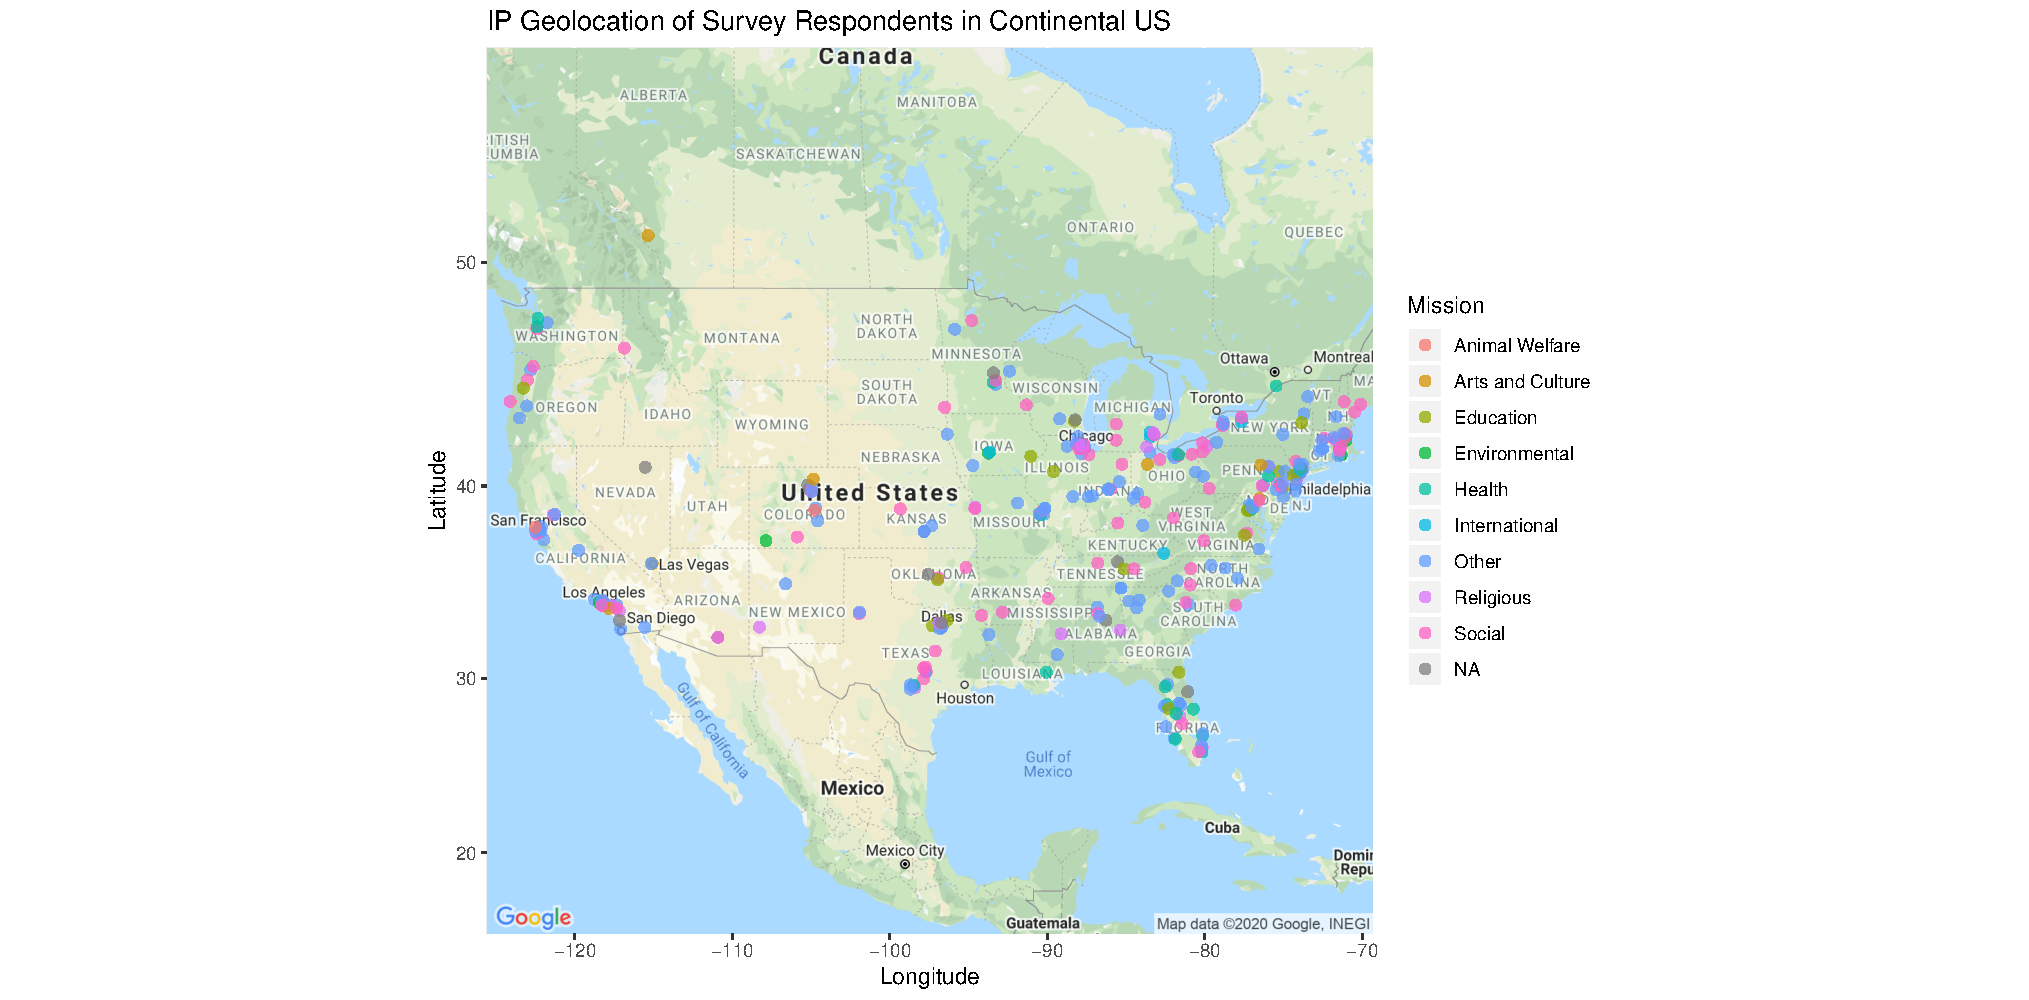
\includegraphics[width=.9\columnwidth]{surveymap.pdf}
\centering
\caption{Geolocation of Respondent IP Addresses}
\label{fig:surveymap}
\end{figure}

Table~\ref{tab:missions} summaries the general issue area provided by respondents who reported a mission area in response to the question: \say{On what mission does your organization spend the most time and money?}\footnote{137 of the respondents answered the question by describing their daily activities. These responses included day-to-day themes such as staff and payroll, as well as big-picture strategic policies, such as outreach.} These missions covered a wide thematic range, from organizations dedicated to \say{Crisis Intervention with Domestic Violence and Sexual Assault victims} to \say{Promoting mutual understanding between the U.S. and Asia} to \say{Making theater accessible to all}, to \say{Preserving the history of Hancock County, Ohio.}
% The missions described by sample respondents included 
 \begin{table}[ht]
 \centering
 \begin{tabular}{rlrr}
   \hline
  & Area & Total & Percent \\
   \hline
 1 & Animal Welfare &   3 & 2.00 \\
   2 & Arts and Culture &  12 & 7.00 \\
   3 & Education &  18 & 10.00 \\
   4 & Environmental &   6 & 3.00 \\
   5 & Health &  22 & 12.00 \\
   6 & International &   9 & 5.00 \\
   7 & Other &   3 & 2.00 \\
   8 & Religious &  17 & 9.00 \\
   9 & Social &  92 & 51.00 \\
    \hline
 \end{tabular}
 \caption{Self-reported mission areas}
 \label{tab:missions}
 \end{table}
 
The sizes of the organizations varied widely, ranging from a self-reported staff of a handful of people to large international organizations. %% Histogram of sizes 

 \begin{table}[ht]
 \centering
 \begin{tabular}{rcc}
   \hline
  Size & Personnel &  Count \\
   \hline
 Micro & 0-2 &112 \\
   Tiny &3-5 & 55 \\
   Small & 6-10 &  43 \\
   Medium & 11-20 &  5 \\
   Large & 21-50 &33 \\
   Very large & 51-100 &  15 \\
   Huge & $\geq$ 101 & 35 \\
    \hline
 \end{tabular}
 \end{table} 
 
\section{Does the transformation theory travel?}

Thus far, this chapter has argued that militant groups and non-profit organizations have a remarkable number of structural similarities. These similarities mean that non-profit managers are likely to also face a personnel resource curse, in which the rank-and-file can pressure leaders into accommodating.

In the remainder of the chapter, I present the results of surveying over 300 self-described non-profit managers for their experiences.  The questions address the points along the process, from admitting personnel who are not in alignment with the mission of the organization, to recruiting more quickly than the organization can accept, and finally to whether the managers experienced rank-and-file members contributing to a changing mission. Although the differences between legal operations and clandestine militant activity would be expected to provide more operating flexibility for leaders of the licit organizations, many of the surveyed leaders report experiencing many of the components of the personnel resource curse as well as upwards-driving pressure for change.

\section{General Views of Leader Accommodation}

To establish how the respondents view leadership, the survey asked a series of questions about respondents' beliefs about the desirability of having leaders of an organization accommodate the preferences of the rank-and-file. The majority of the survey respondents shared the expected view that recruits should be assimilated rather than accommodated. When asked in general about their views on accommodation the interests of new staff, respondents were largely not favorable to the idea of adjusting goals and mission to reflect the preferences of new members. 

The general unwillingness to change the mission of their organization to accommodate the preferences of staff and members also extended to a general aversion to the idea of changing the mission of a hypothetical organization in order to grow.  A slight majority (195) of respondents disagreed with the statement that \say{In order to attract new talent, organizations should be willing to change their goals.}\footnote{16 respondents reported that they \say{agree} with the statement, while 112 \say{Somewhat agree[d].} The respondents who disagreed were less tepid, with 72 reporting that they \say{Disagree} that organizations should change their goals to attract new talent and 123 reporting that they \say{somewhat disagree} with the statement.} Many respondents prescribed top-down management. For example, one noted \say{The changes need to start from the top down, that is how you change the culture of an organization.} Another described effective socialization and post-recruitment selection, saying that \say{the new [staff] that attempted to redirect the mission did not last more than a few weeks. It is important for a non-profit to stick to their mission if they believe in their mission.}

\subsection{Recruitment Outside of Socializing Bandwidth}

The origin of the personnel recruitment curse is recruitment outside of socializing bandwidth. As well, this is the facet of the theory that is puzzling when done by a rational leader. Thus, experiences recruiting outside of their socializing bandwidth is an initial starting point to compare the portability of the transformation theory. Moreover, if the respondents report this behavior, the cross-domain pervasiveness of this recruitment pattern contributes to the puzzle of why a rational leader would violate recruitment best practices. 

The rapid growth of staff is of particular interest because organizations have discretion and agency over their hiring, selection, and intake. This contrasts with the portrayal of many militant and social movements as seeking constant expansion, even at the expense of careful selection, socialization, or internal social endowments or recipients of new members who occasionally \say{flood} the group.\footnote{The former often underlies discussion of the political economy of so-called opportunistic rebel groups or those that expand by kidnapping new members~(\textit{e.g}~\cite{beber2013logic, blattman2010nature, cohen2013female, weinstein2005resources}). The latter framing more common in histories of movements with a nationalist or secessionist motivation. The underlying assumption seems to be that these groups also prioritize expansion, and have not implemented intricate selection and recruitment pipelines. Many of the organizations described in Chapter {[cases]} are of this type.}

The survey posed a series of questions intended to ask whether respondents had experienced personnel growth of staff, members, or the board, that could have challenged the absorption capacity of the organization. Although the bottom-up transformation theory specifically focuses on an expansion that exceeds socializing capacity, the survey concentrated instead on asking about periods of rapid growth, accommodation of the preferences of personnel or members, and short-term decisions that might undermine long-term cohesion.\footnote{The lines of questioning do not directly address recruitment beyond socializing capacity. Questions on this theme elicited a strongly negative reaction during pretesting. Framing questions as socialization failure or internal negotiation were interpreted by respondents as soliciting an admission of leadership failure.}

The results presented below focus on whether the respondent had \say{...ever been part of an organization experiencing a period of rapid growth or personnel change among the staff or the board of directors?} This question revealed a striking frequency of reports of rapid personnel change among staff, with 129 respondents reporting that they had experienced such a period.\footnote{54 respondents denied experiencing such a rapid expansion, with the remainder either giving conflicting responses or failing to answer the question.}

The results are notable for the degree to which rapid expansion of staff was more often reported than rapid recruitment of leaders: only 31 of the respondents reported having experienced quick growth of their Board of Directors and 147 specifically denied having experienced this.\footnote{63 respondents reported having experienced rapid growth on both the board and among the staff. The results are not disambiguated by organization size or general mission area, because the question asked whether the respondent had ever experienced rapid growth among staff, not whether they experienced this in their current organization.}

Of those who reported a rapid staff increase, 37 also responded that they felt that the organization's leadership should have accommodated the preferences of the new base. While only about 10\% of the total respondents, the response nevertheless indicates a sense among practitioners that bottom-up transformation may be beneficial for some organizations. Furthermore, of the 129 respondents who reported experiencing a substantial staff growth, 70 responded that they believed that the result was mission drift in their organizations. 

\subsection{Recruitment of non-aligned personnel}

A second important point of comparison is whether the non-profit leaders reported having recruited personnel who do not share the organizations' mission.

When prompted about recruitment to address specific operational needs, more respondents acknowledged (175) than denied (143) that their organizations had \say{ever needed to recruit people with essential skills or resources, even though their goals were not entirely consistent with those of the organization.} Of those who affirmed that they had needed to recruit for skills or resources rather than mission alignment, 73 responded affirmatively that \say{These personnel changes lead our mission to drift away from the priorities of the leadership.}

Figures~\ref{fig:nonalignedsize} and ~\ref{fig:nonalignedmission} presents the proportion of respondents claiming that their current organization had sought personnel for skills or resources rather than alignment. For ease of interpretation and comparison, the figures present responses clustered according to reported organization size (Figure~\ref{fig:nonalignedsize}) and reported mission (Figure~\ref{fig:nonalignedmission}). Interestingly, the theory laid out in the previous chapters frames the incentive for recruitment as likely originating from weakness and organizational fragility. The weakness pathway suggests that we would expect to see more reports of recruiting personnel with a different mission in smaller organizations. However, for those organizations with a claimed size of under 100 people, the experiences with hiring for skills rather than alignment actually increased as the organizations became larger.
 
\begin{figure}[t]
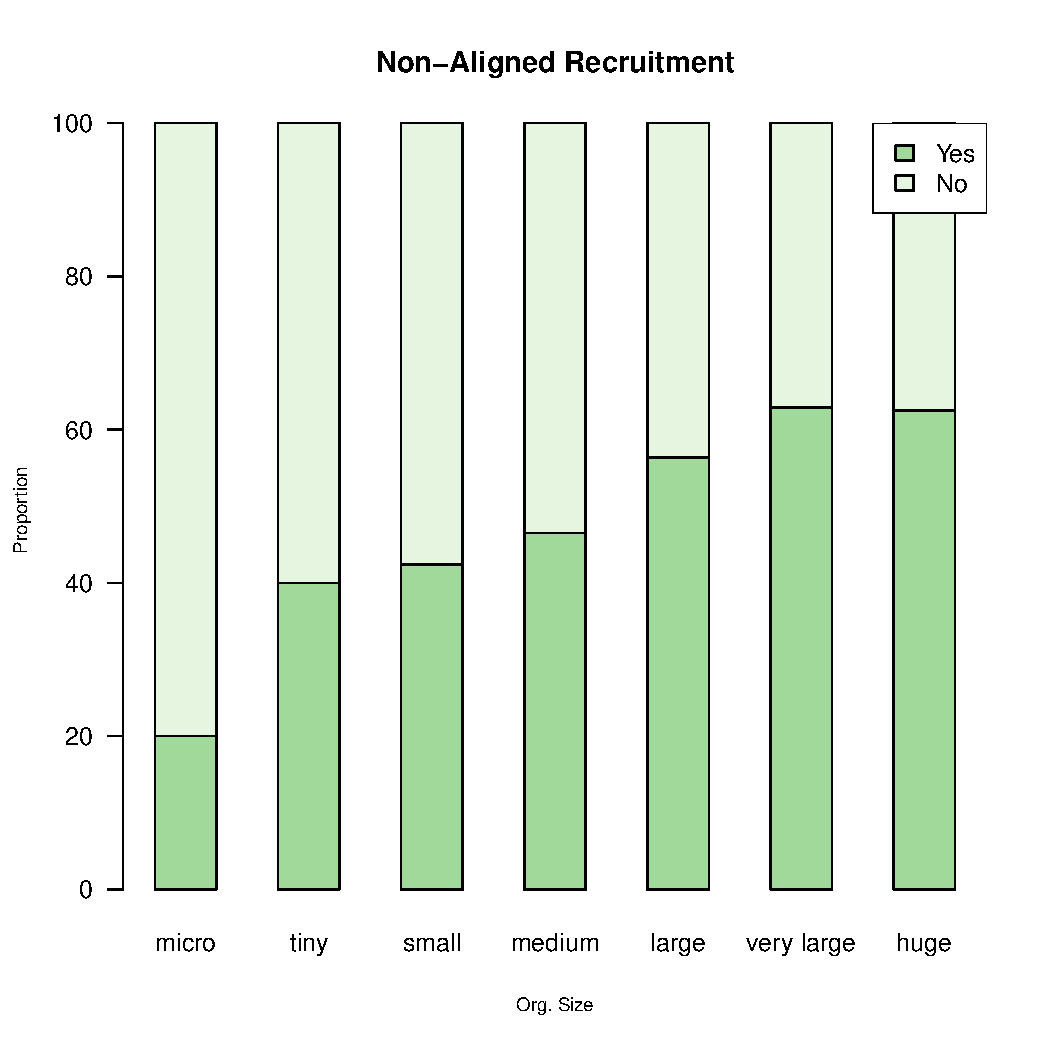
\includegraphics[width=.85\columnwidth]{./Pictures/NonAlignedRecruitmentBySize.pdf}
\centering
\caption{Reports of Recruiting Non-Aligned Staff, by Organization Size}
\label{fig:nonalignedsize}
\end{figure}

The experience with this type of recruitment pattern also changes by the self-reported mission of the respondents. Interestingly, respondents reporting that their organization is primarily involved in health-related issues were most likely to report bringing in non-aligned personnel.\footnote{16 of the 22 respondents claiming a mission that relates to health issues broadly reported this recruiting pattern.} The only individual sector larger than \say{Health} among respondents were the 92 respondents who described a mission that I clustered into the \say{Social} category. Although reporting non-aligned recruitment at a lower rate than those working on health-related issues, more than half (54 out of 92) affirmed that the organization they are part of had followed this recruitment pattern. Conversely, less than half of respondents describing a mission in the \say{Environmental,} \say{International,} and \say{Religious} clusters reported the non-aligned recruitment pattern. 

Although the survey did not ask for insight into the reasons for this recruitment, the over-representation of non-profits working in the technical and highly-licensed health domain may lend support to a pathway for bottom-up transformation that is particularly fast when personnel have hard-to-replicate skills.

\begin{figure}[t]
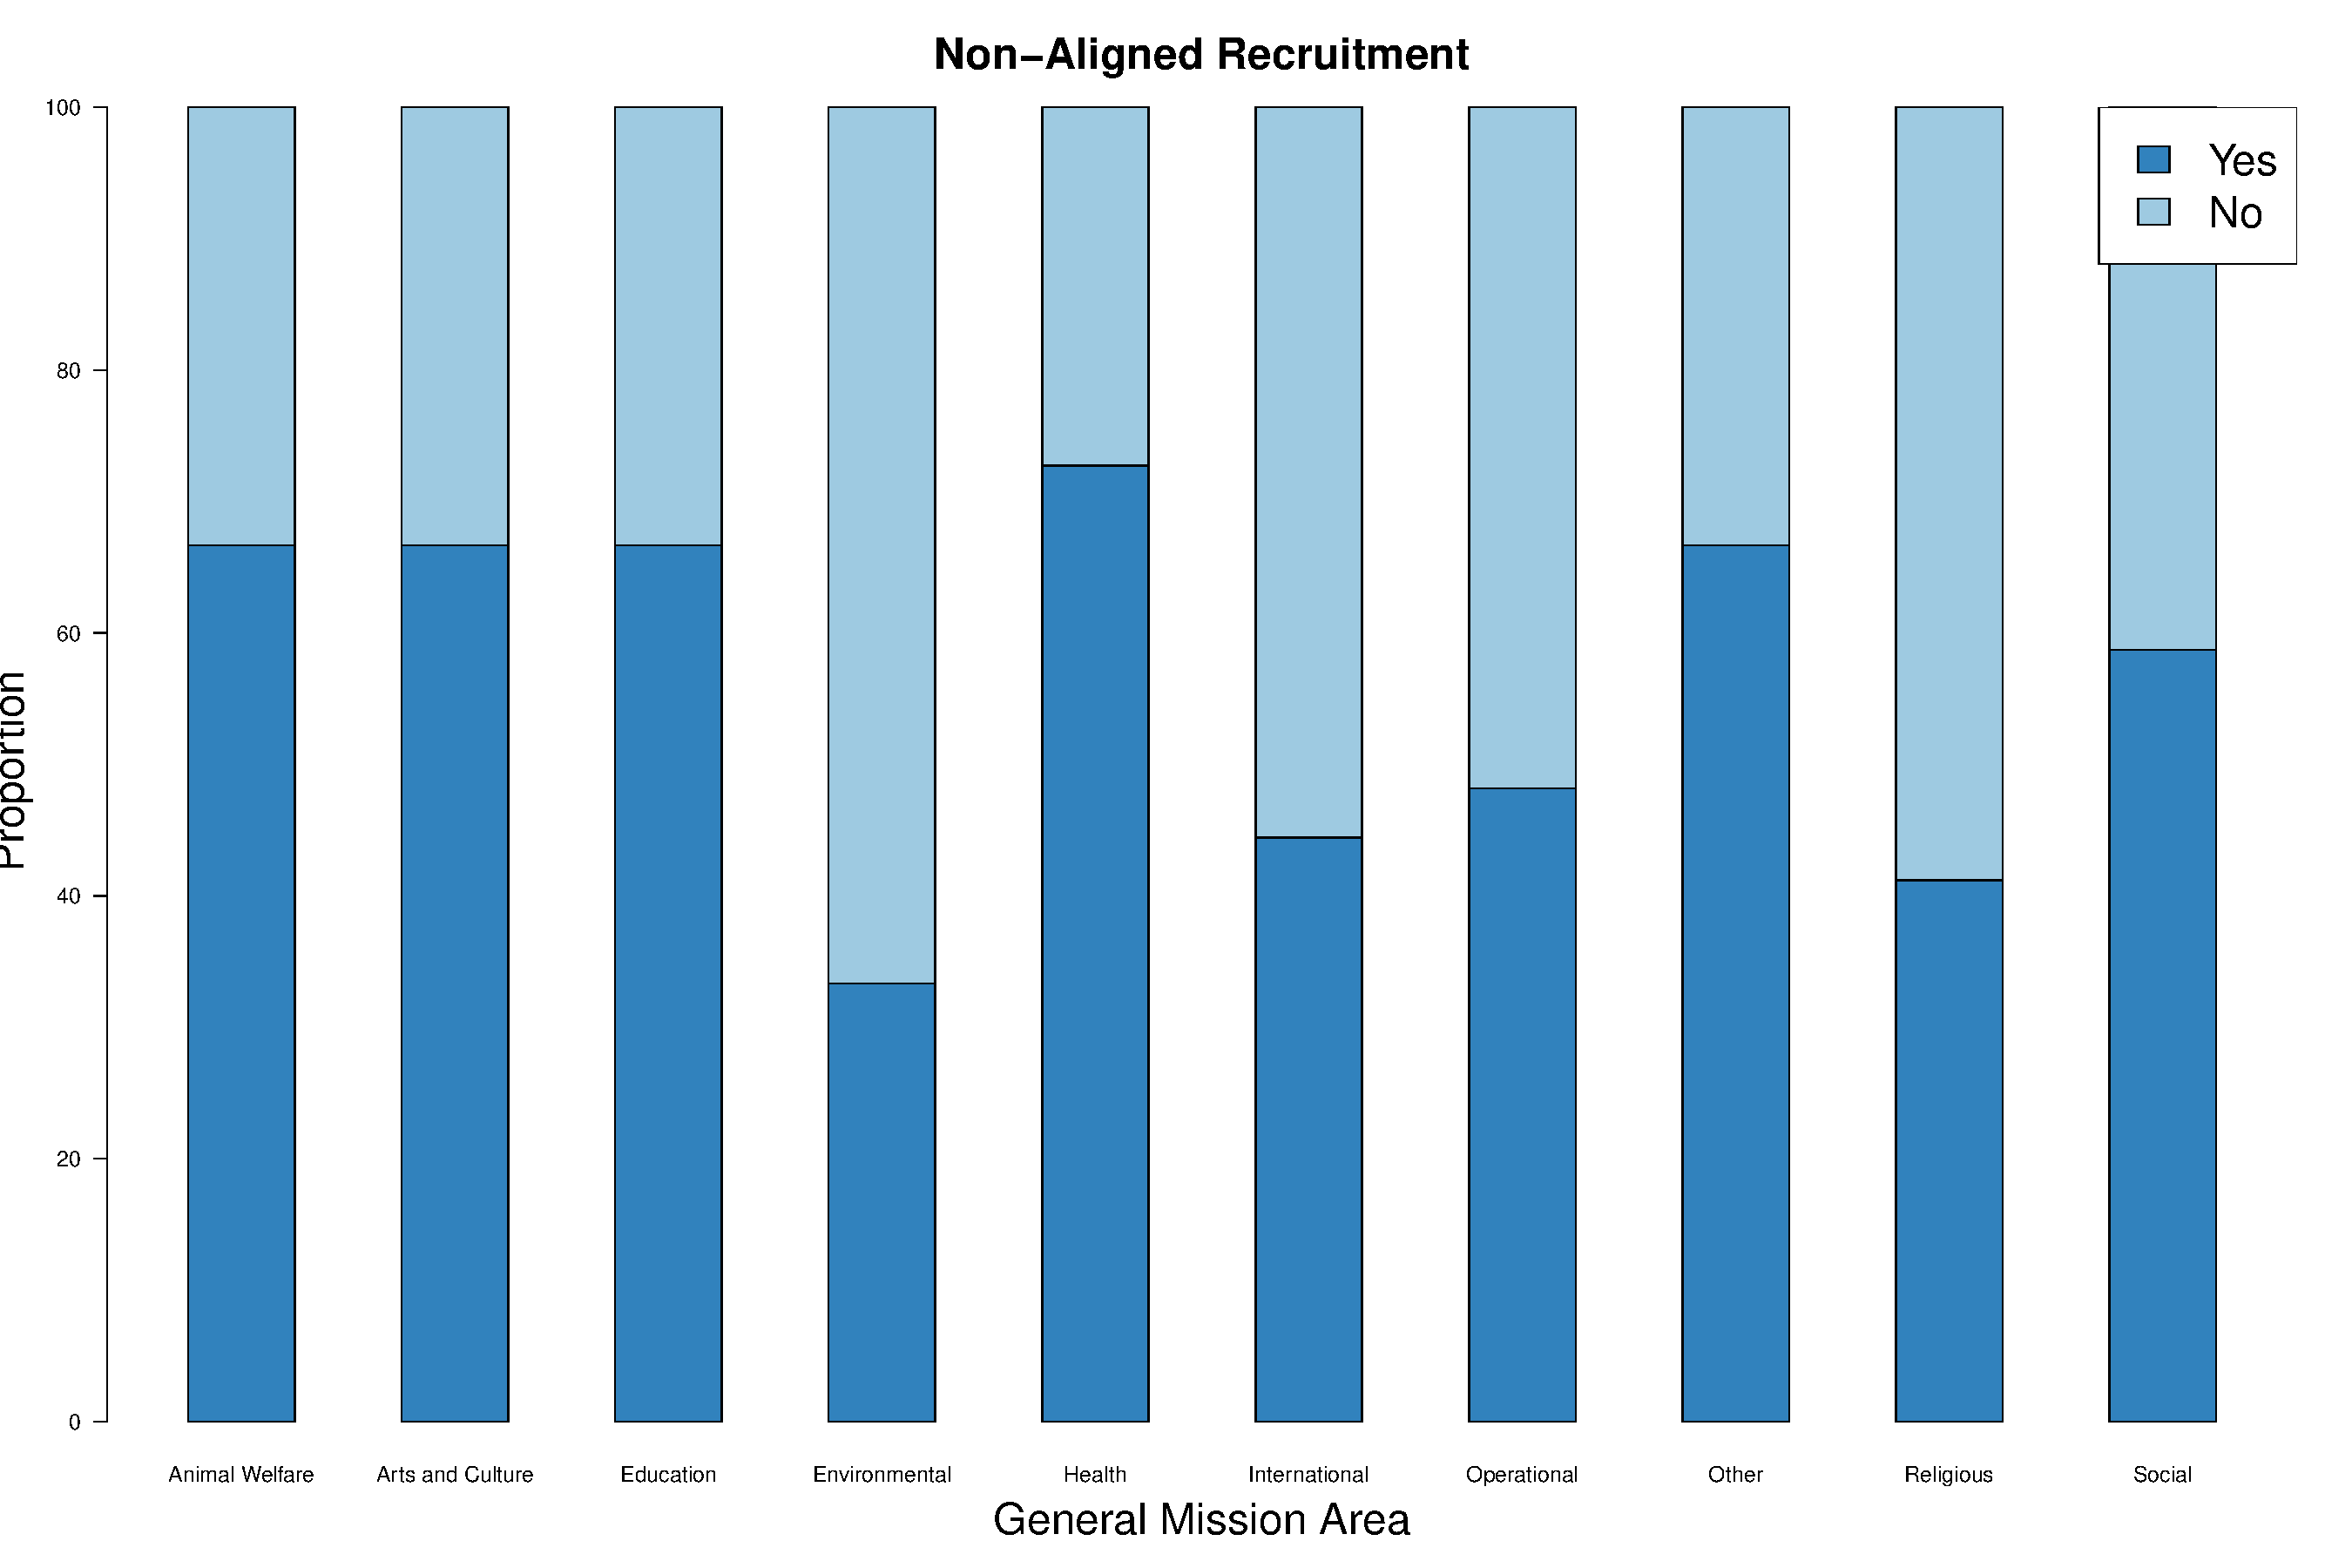
\includegraphics[width=.99\columnwidth]{./Pictures/NonAlignedRecruitmentByMission.pdf}
\centering
\caption{Reports of Recruiting Non-Aligned Staff, by Organization Mission}
\label{fig:nonalignedmission}
\end{figure}

Of those respondents who answered that their organizations had recruited personnel for reasons other than mission alignment, the survey asked whether they believed that the new personnel lead to mission drift in the organization. Of the 156 responses, 68, or 44\%, reported that they either \say{agree[d]} or \say{somewhat agree[d]} that the recruitment of non-aligned personnel resulted in mission drift. 
\subsection{Accommodation Outcome}

Among the survey takers who agreed that they had sought personnel for skills or resources rather than mission alignment, those respondents who reported that their organizations had 6-10 staff members were more likely to report subsequent mission drift caused by the personnel.\footnote{Respondents who said that they had recruited personnel for skills or resources rather than alignment were subsequently asked \say{How strongly, if at all, do you agree or disagree with the statement: \say{These personnel changes lead our mission to drift away from the priorities of the leadership?}}} The rates at which respondents reported mission drift after recruiting staff for skills or resources rather than mission alignment can be seen in Figure~\ref{fig:nonalignedMDsize}, which presents results classified according to the self-reported organizational size.

\begin{figure}[t]
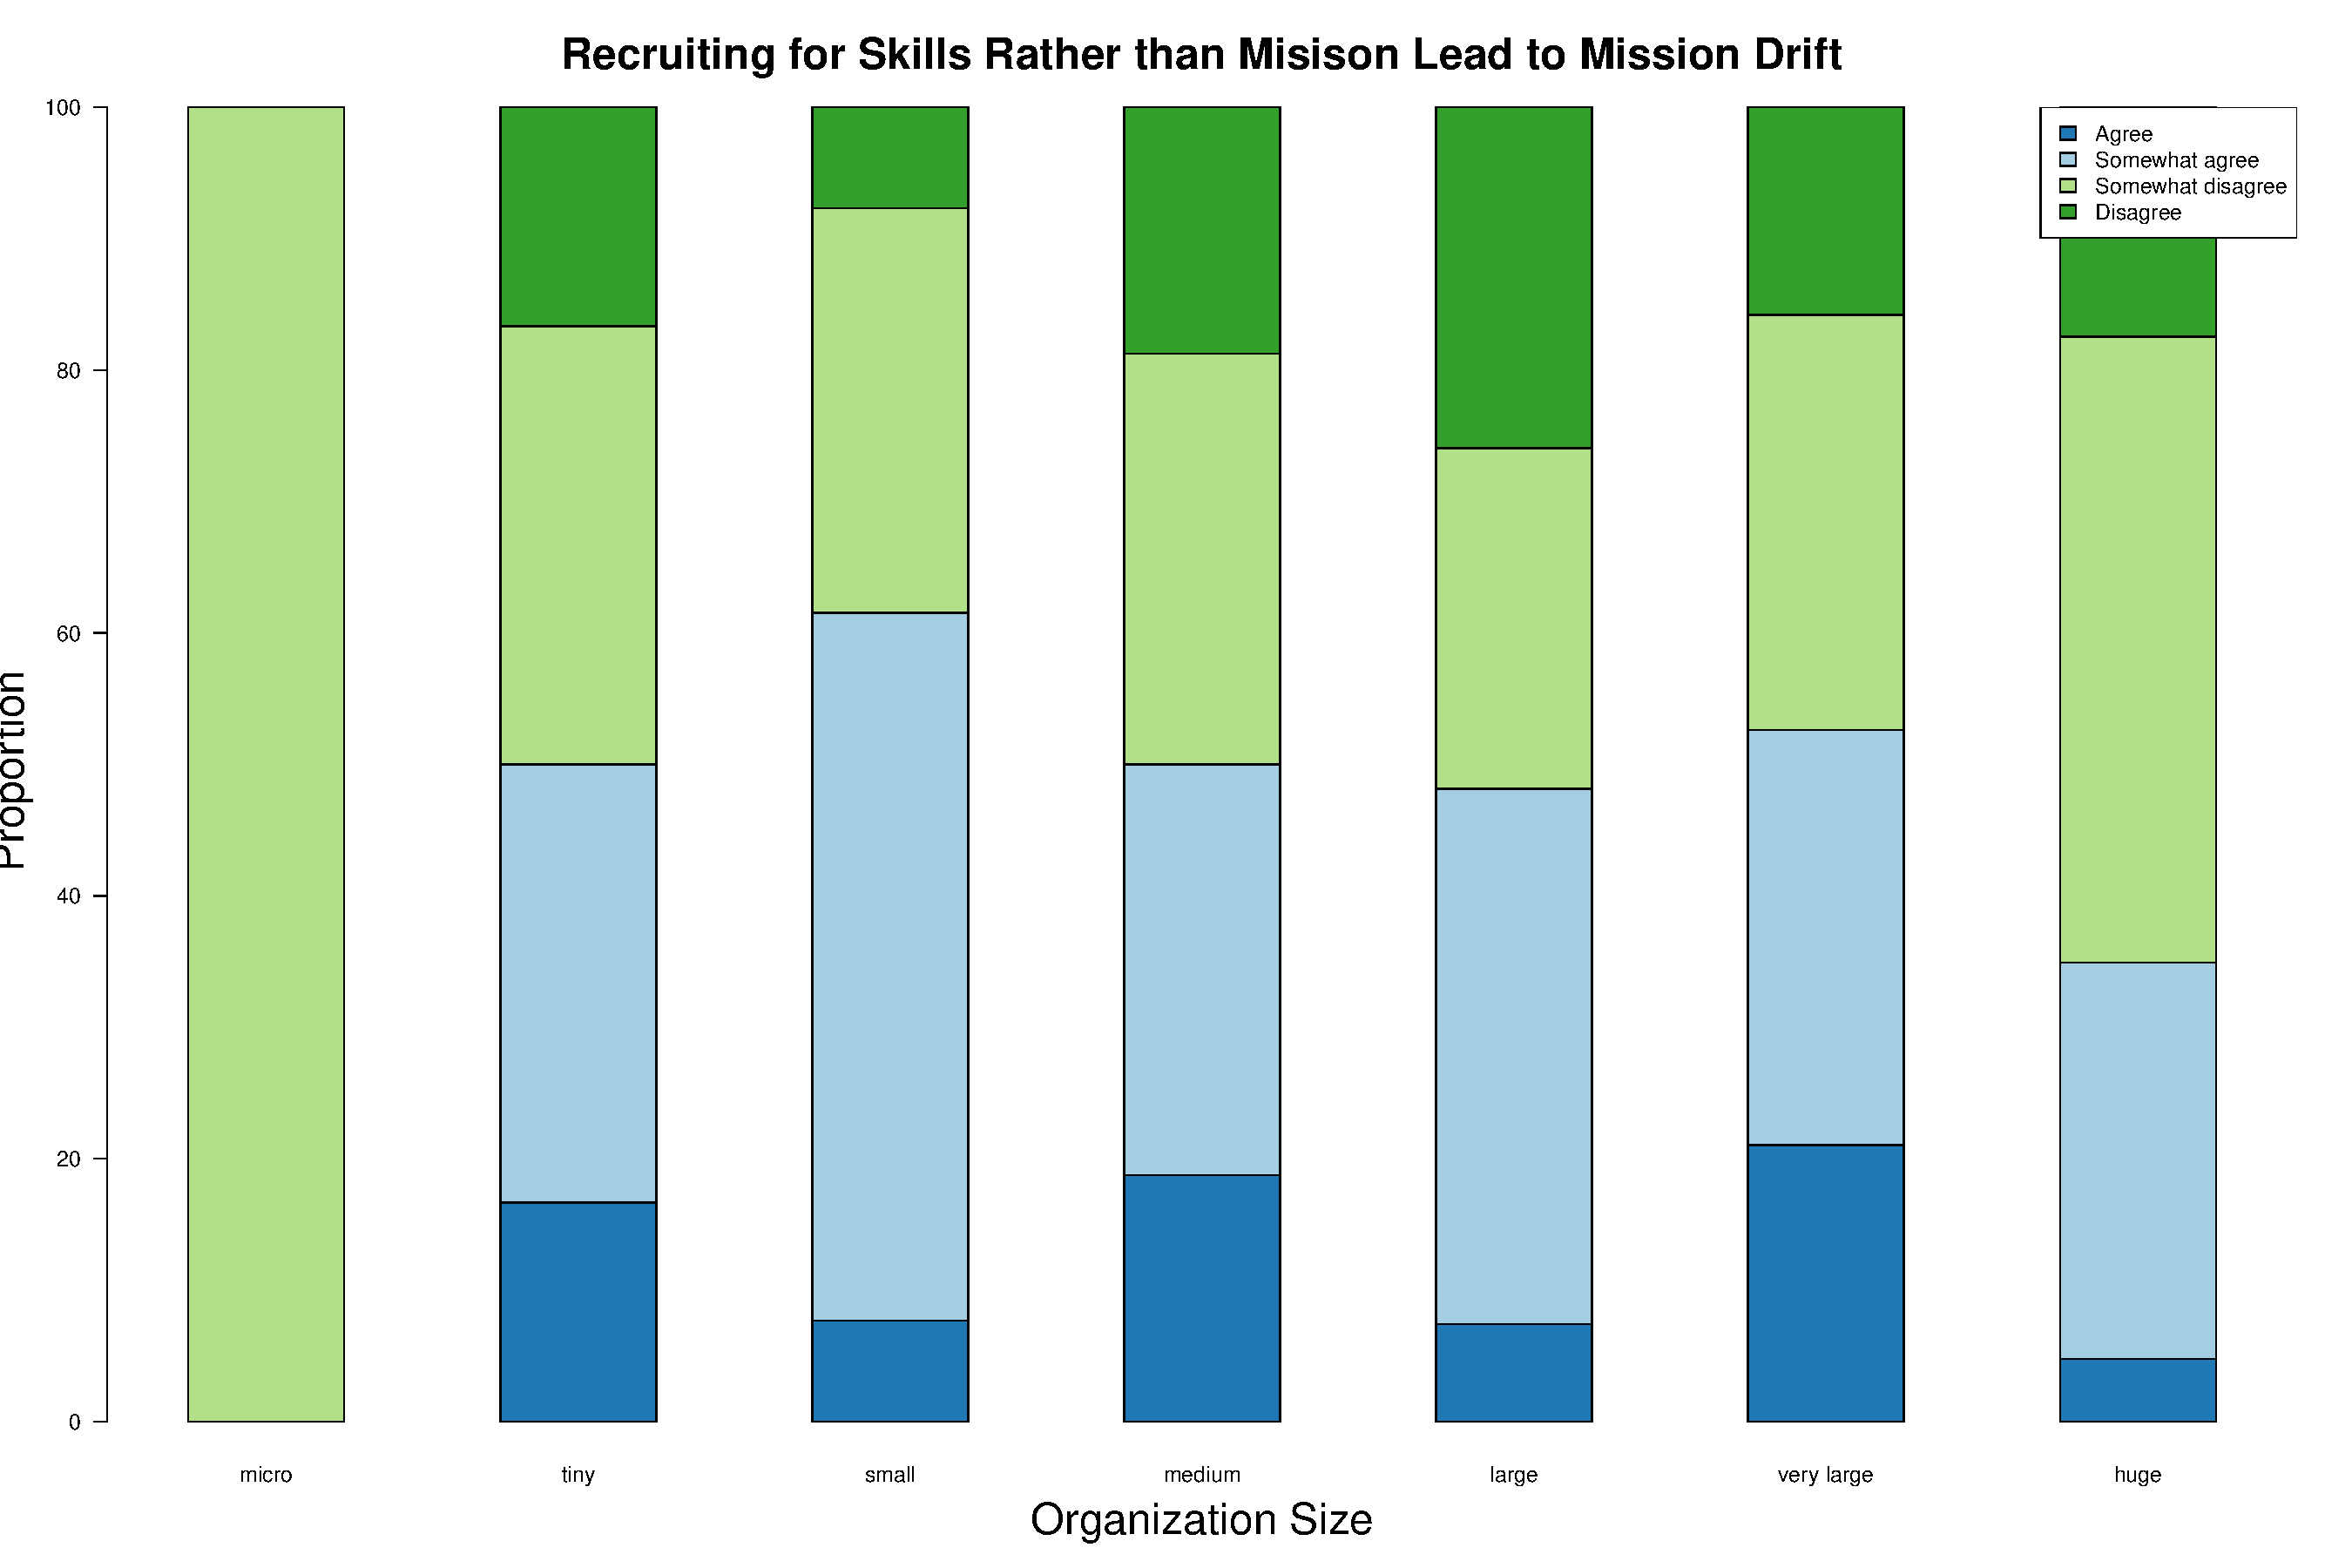
\includegraphics[width=.85\columnwidth]{./Pictures/NonAlignedRecruitmentMDSize.pdf}
\centering
\caption{Mission Drift After Recruitment, by Organization Size}
\label{fig:nonalignedMDsize}
\end{figure}

Although the \say{health} cluster reported the most recruitment of non-mission aligned personnel, they reported this personnel-driven mission drift at lower rates than Arts and Culture or Educational organizations. Figure~\ref{fig:nonalignedMD} presents the percentages of respondents in each cluster of missions who, after agreeing that their organizations had recruited for skills or resources rather than buy-in on mission, did or did not agree that mission drift was a downstream result of this recruitment. 

\begin{figure}[t]
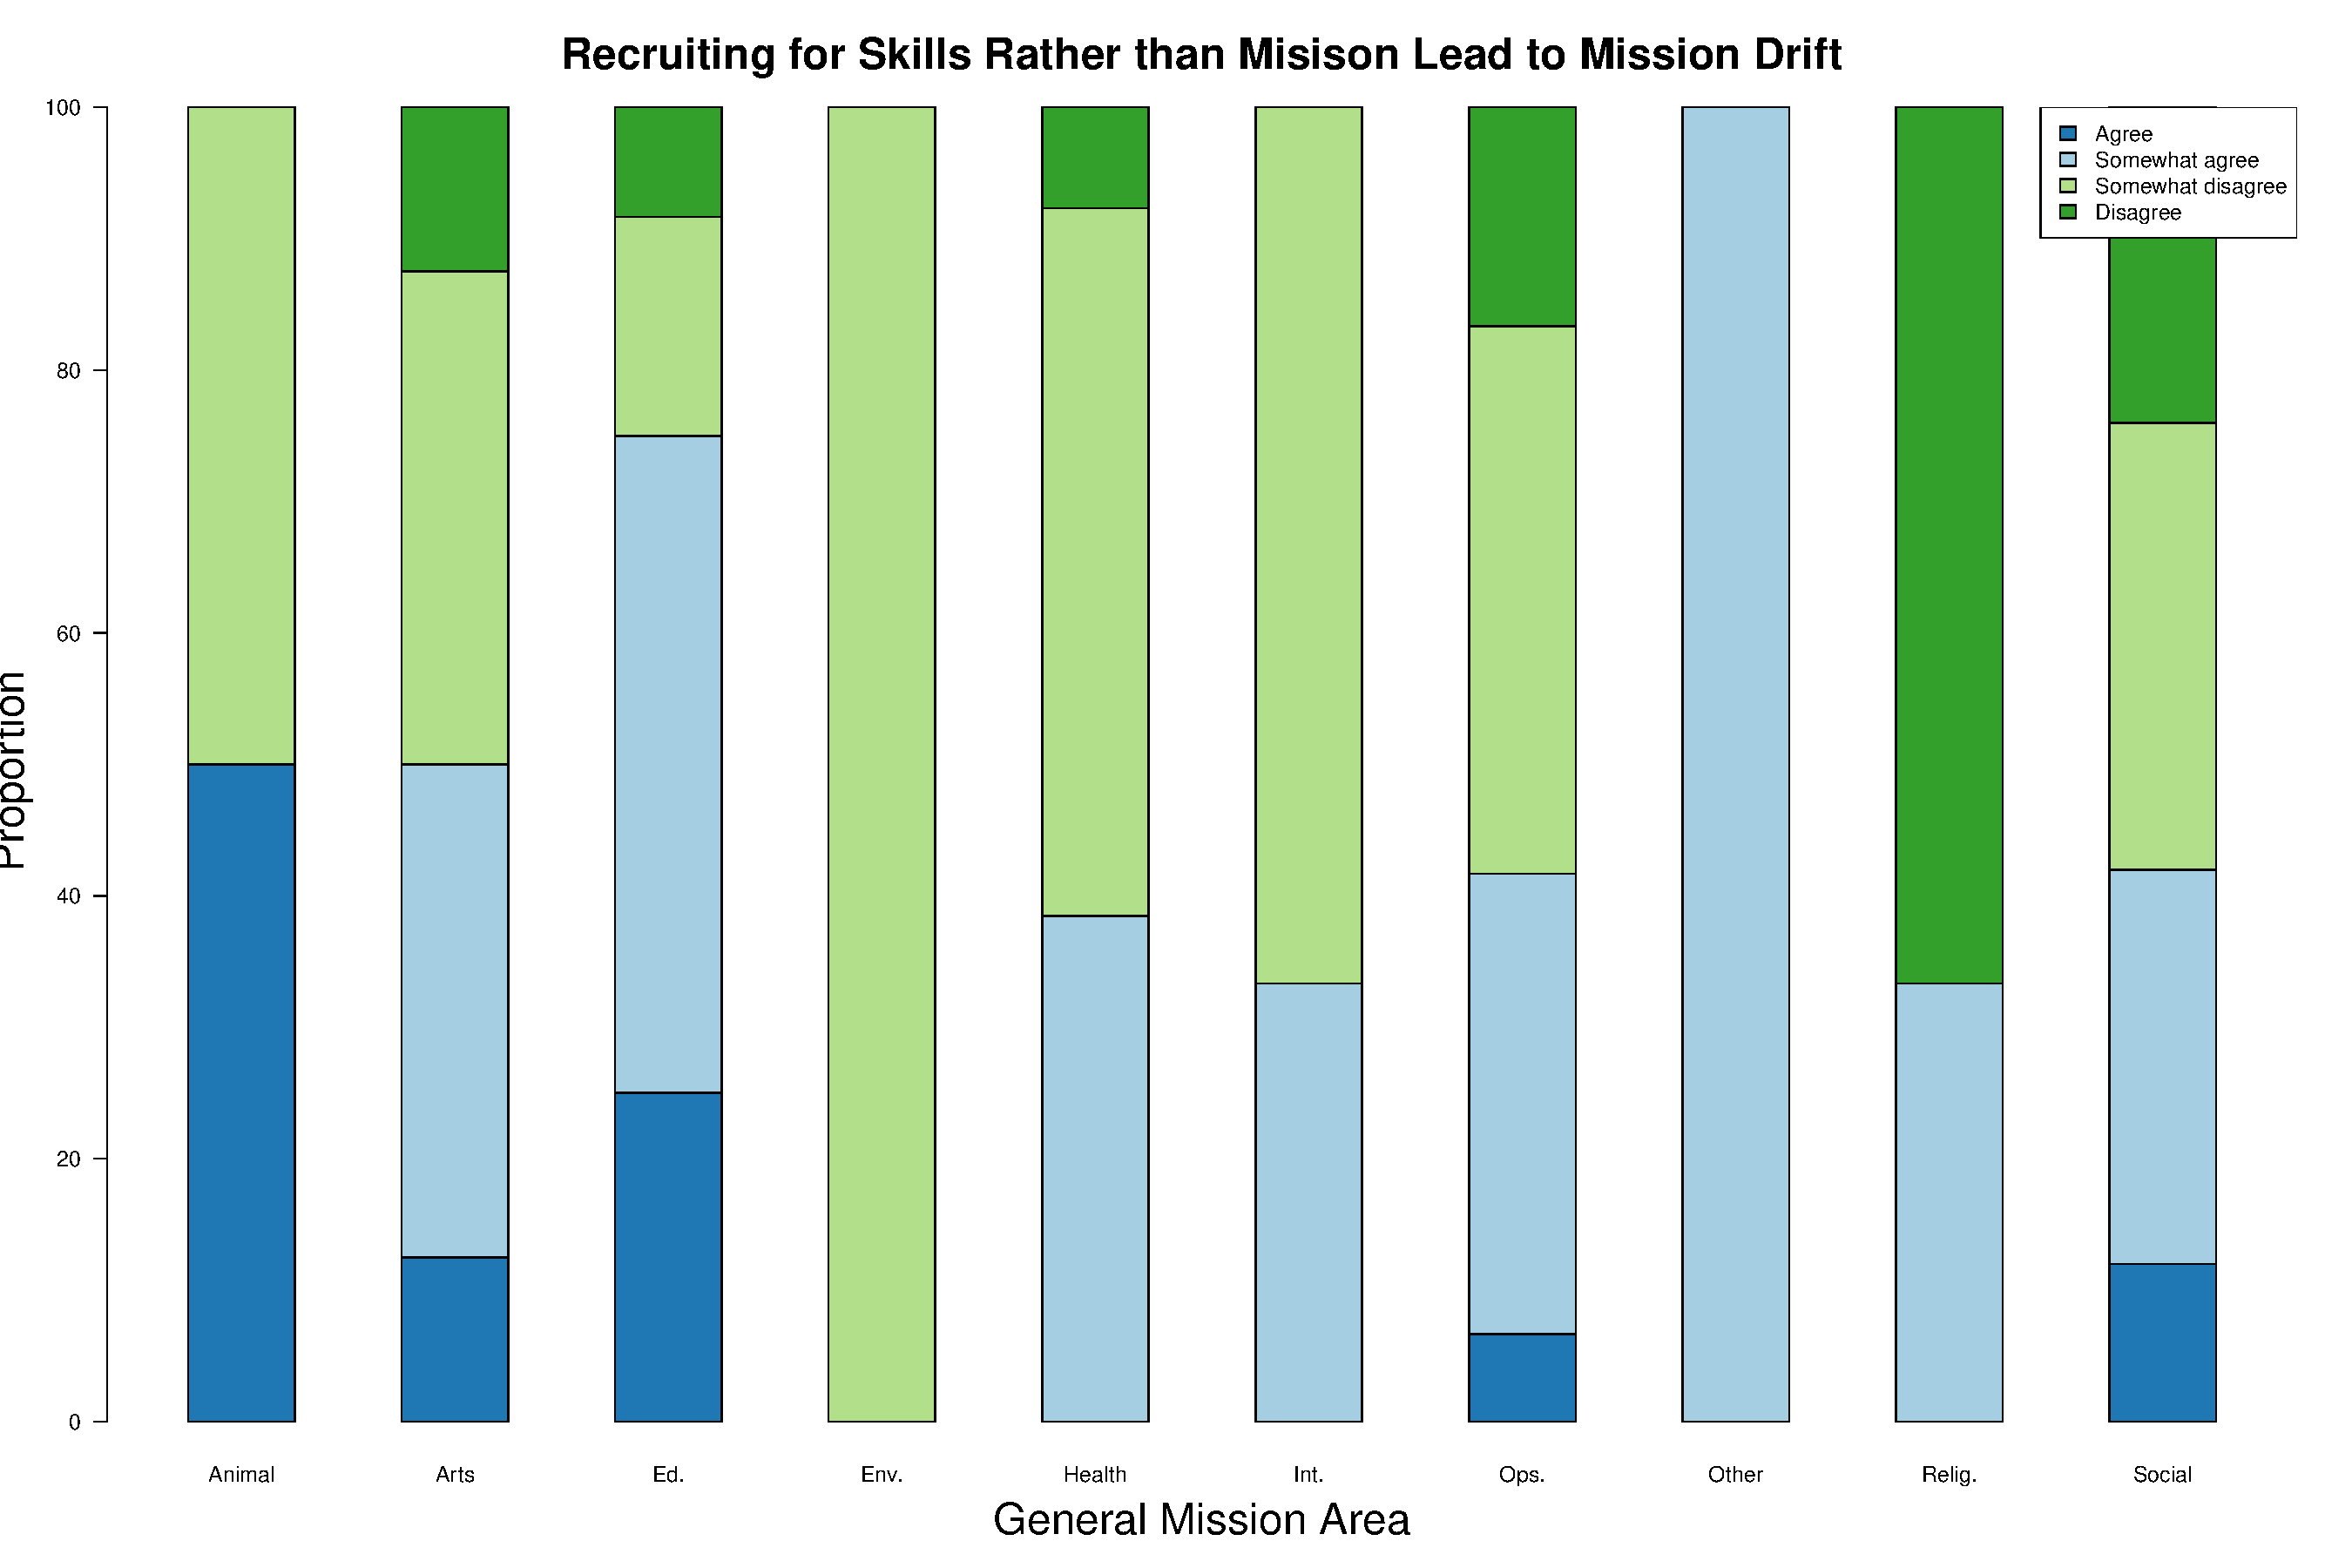
\includegraphics[width=.95\columnwidth]{./Pictures/NonAlignedRecruitmentMD.pdf}
\centering
\caption{Mission Drift After Recruitment, by Type of Mission}
\label{fig:nonalignedMD}
\end{figure}

Survey respondents described their experiences with organizations accommodating new staff. One respondent, located in Miami, noted that in their experience recruiting for skills rather than alignment, the consequence was that \say{changes originated in the changes that were demanded by the members.  The org had to respond or risk losing members.} Another, writing from Southern Maine who identified their organization as a provider of \say{social service [sic],} concluded that the recruitment resulted their group having \say{lost some of our identity} because \say{Changes originated from new staff members who came with their own agenda.} A third--- geolocated to Des Moins, Iowa and reporting that their organization was involved primarily in \say{worldwide missions}--- added: \say{When the staff does not fully embrace and agree with the mission of the organization, then things begin to happen (events, discussions, etc) that begin to steer the organization away from its mission.}

\subsection{Factorial Experiment}

The second half of the survey was designed to test the expectation that leaders can be induced to admit recruits with heterogeneous preferences.  The experiment was administered alongside the non-profit leader survey, and resulted in 291 responses.

The experiment asked respondents to assess two potential candidates for each of a position on the Board of Directors for their organization and a staff role. The conditions included variation on the degree of alignment with the organization. For the potential staff members, the potential personnel also varied in the percentage to which their salary and benefits would be subsidized. These subsidies were either 0, 25\%, 50\%, or 75\%. Potential staff members were characterized as having a preferred mission that was \say{a little different than,} \say{very different than,} and \say{very similar to} the existing mission of the organization. Despite the theory's focus on grassroots organizational members, the experiment included a vignette for potential Board members as well as staff to provide a basis of comparison in how the participants view potential leaders. 

As salaries and benefits are not salient for members of a Board of Directors, prospective Board members varied on whether they would \say{bring needed professional skills} to the Board. Both vignettes noted that \say{You expect that if they join, they will try to steer the organization's mission to align with their goals.} This phrase was included to underscore the expectation that a forward-looking leader would recruit new personnel even knowing that the new staff will attempt to change the direction of the organization, 

The factorial design instructed the respondents to consider that the organization that they were hiring for had a resource level that was ~\say{secure and stable},~\say{barely sufficient}, or~\say{precarious— not sure if operations will continue}. This feature connected the prompt from the factorial to the expectation that survival pressures would induce leaders to accept potential staff or board member with preferences further from their existing mission.

The vignettes thus presented a menu of potential staff or Board members, an accompanying resource or skill inducement, and an underlying condition of scarcity. Without influence of the resource or skill inducements, respondents should gravitate towards those candidates whose preferences are \say{very similar to} those of their organizations. If external subsidies can induce leaders to admit recruits with heterogeneous preferences, selection of staff or potential board members with different preferences should increase in the promised skills or salary subsidy. 

The degree to which each condition contributed to respondent preferences can be seen in Figure~\ref{fig:factorial}, plotted via the Cregg package for R~\autocite{leeper2018cregg}. The Marginal Mean plot depicts the impact of each condition on the likelihood of respondents choosing a candidate with each trait. Values above 0.5 indicate features that increase the profile's likelihood to be selected, while those below 0.5 decrease the profile's propensity to be selected.  In assessing individual features, the survey respondents were consistently most likely to select a candidate described as having a mission preference very close to the organization. Although the experiment results do not reflect the expectation of the formal model, the results underscore the degree to which rapid recruitment of members with heterogeneous preferences occurs despite, rather than because of, leader preferences.

%% Looking for any combinations in the factorial that show that they do have
%% some kind of trade-off (is there any pair of things that are interesting and suggestively  supportive)

\begin{figure}[t]
\centering
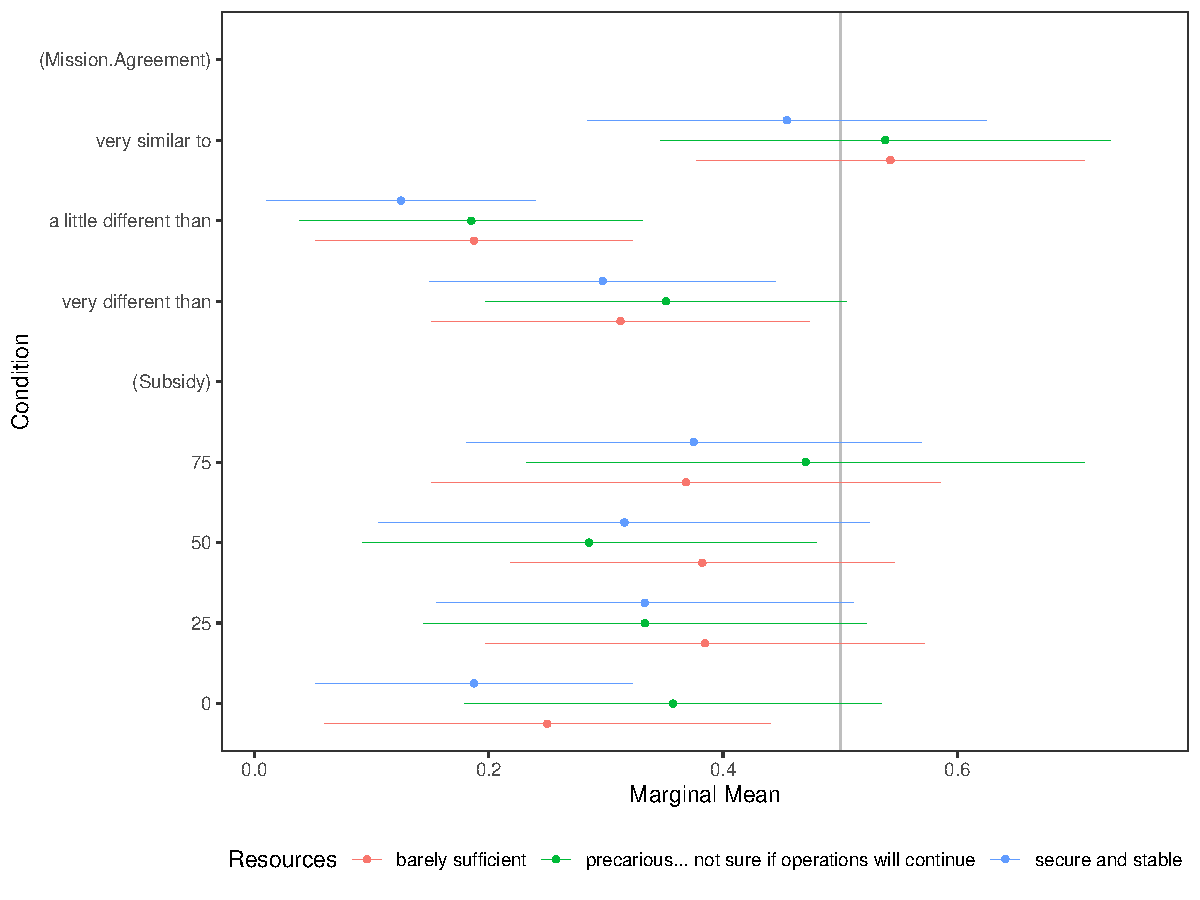
\includegraphics[width=.85\columnwidth]{./Pictures/simpleConjoint.pdf}
\caption{Baseline Results of Factorial Experiment}
\label{fig:factorial1}
\end{figure}


%% Summarize that in the morning of 2/24


\section{Conclusion}

This chapter has sought to demonstrate that the core insights that drive the Personnel Resource Curse apply in domains other than the militant groups that have formed the focus of previous chapters of the dissertation. It has had twofold goals. First, to demonstrate that the apparently-puzzling behavior of organizational leaders accepting large numbers of new personnel whom they will be unable to socialize into the existing mission is not a pathology specific to the operational demands of militant groups. 

The first goal is important to expand the theory outside of the domain of militant groups. Finding cross-domain applications of the theory has important implications. First, finding similar behavioral patterns in a separate domain is reassuring for the framing of the Personnel Resource Curse as a general theory of organizational change. 

Second, it provides an independent domain in which to test the predictions of the theory, and thereby provides an opportunity to avoid circular reasoning of using the same cases and domain both for theory development and testing. This builds on the work of scholars who have argued that militant groups are not completely \textit{sui generis} and can thus be analyzed and countered using conceptual tools developed in other domains.

The chapter presented the results of asking non-profit leaders and managers whether they had ever experienced a rapid intake of personnel that do not share the organization's original mission in order to demonstrate that the initial recruitment shock that initiates the process is not unique to militant or clandestine groups. The finding that a substantial minority of the respondents had experienced this type of growth provides a strong signal that this organizational pattern is not an idiosyncrasy of militant groups. As well, it gives an initial estimate of the frequency at which organizations may experience recruitment shocks that result in downstream consequences. 

It provides support for the specific theory of upward-driving organizational change by establishing that among the sample of non-profit leaders surveyed, there is a non-trivial baseline belief that they have experienced mission-drift after recruitment. Experiences with bottom-up mission drift were reported alongside claims that change should originate with leaders and that new recruits should conform to their new organizations. This parallel's the theory's expectations that bottom-up transformation should occur despite, not because of, leader preferences.

Finally, the chapter presented a factorial experiment designed to test the prediction from the formal model that leaders can be induced by circumstances to recruit non-aligned members even knowing that they will eventually have to accommodate their preferences. The experiment focused on whether the combination of organizational precarity and external subsidies could induce leaders to knowingly hire either staff or board members that would try to change the organization. The results did not support the expectation that those leaders who were presented with a situation of resource scarcity would be more willing to hire new staff who did not align with their mission. This finding may be consistent with the observation that the rapid recruitment is a feature of many organizational histories, despite being against recruitment best practices.  When presented with an abstract condition, the leaders were uninterested in recruiting new personnel who would attempt to redirect the group, even with the dual inducements of financial stress and a deep discount on the prospective member. 




